\documentclass[11pt]{article}
%\usepackage{fullpage,graphicx,algorithm,algorithmic,bm,amsmath,amsthm,amssymb,color,hyperref,cite,natbib}

% if you need to pass options to natbib, use, e.g.:
%\PassOptionsToPackage{numbers}{natbib}
\usepackage{natbib}
\usepackage{bm,amsmath,amsthm,amssymb,multicol,algorithmic,algorithm,enumitem}
\usepackage{wrapfig,lipsum}
\usepackage[textwidth=1cm,textsize=footnotesize]{todonotes}

% ready for submission
\usepackage{neurips_2020}

\usepackage[colorlinks=true,
linkcolor=red,
urlcolor=blue,
citecolor=blue]{hyperref}
\usepackage{hyperref}
\usepackage{cleveref}

\setlength{\parskip}{.2cm}

\newtheorem{Fact}{Fact}
\newtheorem{Lemma}{Lemma}
\newtheorem{Prop}{Proposition}
\newtheorem{Theorem}{Theorem}
\newtheorem{Def}{Definition}
\newtheorem{Corollary}{Corollary}
\newtheorem{Conjecture}{Conjecture}
\newtheorem{Property}{Property}
\newtheorem{Observation}{Observation}
%\theorembodyfont{\rmfamily}
\newtheorem{Exa}{Example}
\newtheorem{assumption}{H\!\!}
\newtheorem{assumptionA}{S\!\!}
\newtheorem{assumptionL}{L\!\!}
\newtheorem{Remark}{Remark}
\newtheorem*{Lemma*}{Lemma}
\newtheorem*{Theorem*}{Theorem}
 \makeatletter
\renewenvironment{proof}[1][\proofname]{%
   \par\pushQED{\qed}\normalfont%
   \topsep6\p@\@plus6\p@\relax
   \trivlist\item[\hskip\labelsep\bfseries#1]%
   \ignorespaces
}{%
   \popQED\endtrivlist\@endpefalse
}
\makeatother

%%%%%%%%%%% Stuffs for Tikz %%%%%%%%%%%%%%%%%%
\usepackage{pgfplots}
\usepackage{xargs}
\usepackage{stmaryrd}
\usetikzlibrary{arrows,shapes,calc,tikzmark,backgrounds,matrix,decorations.markings}
\usepgfplotslibrary{fillbetween}

\pgfplotsset{compat=1.3}

\usepackage{relsize}
\tikzset{fontscale/.style = {font=\relsize{#1}}
    }

\definecolor{lavander}{cmyk}{0,0.48,0,0}
\definecolor{violet}{cmyk}{0.79,0.88,0,0}
\definecolor{burntorange}{cmyk}{0,0.52,1,0}

\def\lav{lavander!90}
\def\oran{orange!30}

\definecolor{asuorange}{rgb}{1,0.699,0.0625}
\definecolor{asured}{rgb}{0.598,0,0.199}
\definecolor{asuborder}{rgb}{0.953,0.484,0}
\definecolor{asugrey}{rgb}{0.309,0.332,0.340}
\definecolor{asublue}{rgb}{0,0.555,0.836}
\definecolor{asugold}{rgb}{1,0.777,0.008}

%%%%%%%%%%%%%%%%%%%%%%%%%%%%%%%%%%%%%


\usepackage{shortcuts_OPT}

%\renewcommand{\textwidth}{5.5in}

% Here's the definition of Sb, stolen from amstex
    \makeatletter
    \def\multilimits@{\bgroup
  \Let@
  \restore@math@cr
  \default@tag
 \baselineskip\fontdimen10 \scriptfont\tw@
 \advance\baselineskip\fontdimen12 \scriptfont\tw@
 \lineskip\thr@@\fontdimen8 \scriptfont\thr@@
 \lineskiplimit\lineskip
 \vbox\bgroup\ialign\bgroup\hfil$\m@th\scriptstyle{##}$\hfil\crcr}
    \def\Sb{_\multilimits@}
    \def\endSb{\crcr\egroup\egroup\egroup}
\makeatother

\newtheoremstyle{t}         %name
    {\baselineskip}{2\topsep}      %space above and below
    {\rm}                   %Body font
    {0pt}{\bfseries}  %Heading indent and font
    {}                      %after heading
    { }                      %head after space
    {\thmname{#1}\thmnumber{#2}.}

\theoremstyle{t}
\newtheorem{q}{Q}
\parindent=0pt

%\newcommand{\eric}[1]{\todo[color=red!20]{{\bf EM:} #1}}
%\newcommand{\erici}[1]{\todo[color=red!20,inline]{{\bf EM:} #1}}
%\newcommand{\belhal}[1]{\todo[color=green!20]{{\bf BK:} #1}}
%\newcommand{\belhali}[1]{\todo[color=green!20,inline]{{\bf BK:} #1}}
%\newcommand{\toco}[1]{\todo[color=yellow!20]{{\bf To:} #1}}



\makeatletter
\DeclareRobustCommand*\cal{\@fontswitch\relax\mathcal}
\makeatother

\begin{document}
% \title{Distributed and Private Stochastic EM Methods\\
% via Quantized and Compressed MCMC}
\title{Distributed and Private Stochastic EM Methods}
%\author{}
\date{\today}

\maketitle

\begin{abstract}
To be completed
\end{abstract}


\section{Introduction}

We consider the distributed minimization of the following negated log incomplete data likelihood 
\begin{align} \label{eq:em_motivate}
\begin{split} 
 \min_{ \theta \in \Theta }~ \overline{L} ( \theta ) \eqdef  L ( \theta ) + r (\theta) \quad \text{with}~~L(\theta) = \frac{1}{n} \sum_{i=1}^n L_i( \theta) \eqdef  \frac{1}{n} \sum_{i=1}^n \big\{ - \log g( y_i ; \theta ) \big\}\eqs,
\end{split} 
\end{align}
where $n$ denotes the number of workers, $\{y_i\}_{i=1}^n$ are observations, $\theta \subset \rset^d$ is the parameters set and $\Pen : \theta \rightarrow \rset$ is a smooth regularizer.

The objective  $L( \theta )$ is possibly {nonconvex} and is assumed to be lower bounded. 
In the latent data model, the likelihood $g(y_i ; \theta)$, is the marginal distribution of the complete~data likelihood, noted $f(z_i,y_i; \theta)$, such that 
\begin{align}
g(y_i; \theta) = \int_{\Zset} f (z_i,y_i;\theta) \mu(\rmd z_i),    
\end{align}
where $\{ z_i \}_{i=1}^n$ are the vectors of latent variables associated to the observations $\{y_i\}_{i=1}^n$.

We also consider a special case of that problem since the complete likelihood pertains to the curved exponential family:
\beq \label{eq:exp}
f(z_i,y_i; \theta) = h  (z_i,y_i) \textrm{exp} ( \pscal{S(z_i,y_i)}{\phi(\theta)} - \psi(\theta) )\eqs,
\eeq
where $\psi(\theta)$, $h(z_i,y_i)$ are scalar functions, $\phi(\theta) \in \rset^k$ is a vector function, and $\{S(z_i,y_i) \in \rset^k\}_{i=1}^n$ is the vector of sufficient statistics.
We refer the readers to \citep{efron1975defining} for details on this subclass of problems which is of high interest given the broad range of problems that fall under this assumption.
In the centralized settings, \ie when all data points are stored in a central server, a reference tool for learning such a model is called the EM algorithm~\citep{dempster1977Maximum, wu1983convergence}. Comprised of two steps, the E-step computes an aggregated sum of expectations as follows:

\beq \label{eq:estep}
\overline{s}(\theta) = \frac{1}{n}\sum_{i=1}^n \overline{s}_i(\theta) \quad \textrm{where} \quad \overline{s}_i(\theta) \eqdef \int_{\Zset} S(z_i,y_i) p(z_i|y_i;\theta) \rmd z_i \eqsp,
\eeq

and the {M-step} is given by
\begin{align}\label{eq:mstep}
\overline{\theta}( \overline{s}(\theta) ) \eqdef \argmin_{ \vartheta \in \theta } ~\big\{ r( \vartheta ) + \psi( \vartheta) - \pscal{ \overline{s}(\theta)}{ \phi ( \vartheta) } \big\} \eqsp.
\end{align}

\subsection{Our motivations}

\textbf{Expectations are not tractable:} Sampling for those approximations are costly.


\textbf{Need for distributed computing: } MovieLens, Large n, compute time, decentralized infrastructure


\textbf{Need for privacy and communication efficiency: } Sensible data (hospital, user data...) that can not be moved. Low bandwidth devices (compute should be light).


\subsection{Our contributions}

%\subsection{Periodic averaging of the local models}
%
%\begin{algorithm}[H]
%\caption{FL-SAEM with parameter averaging} \label{alg:flsaem}
%\begin{algorithmic}[1]
%%\small
%\STATE \textbf{Input}: .
%\STATE Init: $\theta_{0} \in \Theta \subseteq \mathbb R^d $, as the global model and $\bar{\theta}_0 =  \frac{1}{n} \sum_{i=1}^n \theta_0$.
%\FOR{$r=1$ to $R$}
%\FOR{parallel for device $i \in D^{r}$}
%\STATE Set $\hat{\theta}^{(0,k)}_i = \hat{\theta}^{(k)}$.
%\FOR{$t=1$ to $T$}
%\STATE Draw M samples $\{z_{i,m}^{(t,k)}\}_{m=1}^{M}$ under model $\hat{\theta}^{(t,k)}_i$
%\STATE Compute the surrogate sufficient statistics $\tilde{S}_{i}^{(t,k+1)}$
%\STATE Update local model:
%$$
%\hat{\theta}^{(t,k+1)}_i = \overline{\theta}( \tilde{S}_i^{(t,k+1)}) 
%$$
%\ENDFOR
%\STATE Devices send $\hat{\theta}^{(T,k+1)}_i$ to server.
%\ENDFOR
%\STATE Server computes \textbf{the average of the local models}:
%$$
%\hat{\theta}^{(k+1)} = \frac{1}{n} \sum_{i=1}^n \hat{\theta}^{(T,k+1)}_i
%$$ 
%and send global model back to the devices. \label{line:final}
%\ENDFOR
%\end{algorithmic}
%\end{algorithm}
%
%
%\subsection{Periodic averaging of the local statistics}
%
%\begin{algorithm}[H]
%\caption{FL-SAEM with statistics averaging} \label{alg:flsaem2}
%\begin{algorithmic}[1]
%%\small
%\STATE \textbf{Input}: .
%\STATE Init: $\theta_{0} \in \Theta \subseteq \mathbb R^d $, as the global model and $\bar{\theta}_0 =  \frac{1}{n} \sum_{i=1}^n \theta_0$.
%\FOR{$r=1$ to $R$}
%\FOR{parallel for device $i \in D^{r}$}
%\STATE Set $\hat{\theta}^{(0,k)}_i = \hat{\theta}^{(k)}$.
%\FOR{$t=1$ to $T$}
%\STATE \textcolor{red}{ Here one local iteration, $T=1$}
%\STATE Draw M samples $z_{i,m}^{(k)}$ under model $\hat{\theta}^{(t,k)}_i$
%\STATE Compute the surrogate sufficient statistics $\tilde{S}_{i}^{(t,k+1)}$
%\ENDFOR
%\STATE Devices send local statistics $\tilde{S}_{i}^{(t,k+1)}$ to server.
%\ENDFOR
%\STATE Server computes \textbf{global model using the aggregated statistics}:
%$$
%\hat{\theta}^{(k+1)} = \overline{\theta}( \tilde{S}^{(t,k+1)}) 
%$$
%where $\tilde{S}^{(t,k+1)} = (\tilde{S}_i^{(t,k+1)}, i \in D_r)$  and send global model back to the devices. 
%\ENDFOR
%\end{algorithmic}
%\end{algorithm}

\clearpage
\section{Related Work}

\textbf{EM algorithms:}

In the case when the computation of the expectation under the posterior distribution is impossible, the Monte Carlo EM (MCEM) has been introduced in~\cite{wei1990monte} where a Monte Carlo (MC) approximation for this expectation is computed. A variant of that algorithm is the Stochastic Approximation of the EM (SAEM) in~\cite{delyon1999} leveraging the power of Robbins-Monro update~\cite{robbins1951stochastic} to ensure pointwise convergence of the vector of estimated parameters using a decreasing stepsize rather than increasing the number of MC samples.
The MCEM and the SAEM have been successfully applied in mixed effects models~\cite{mcculloch1997maximum,hughes1999mixed,baey2016nonlinear} or to do inference for joint modeling of time to event data coming from clinical trials in~\cite{das2010Inferences}, unsupervised clustering in~\cite{ngChoice2003}, variational inference of graphical models in~\cite{BleiVariational2017} among other applications.
An incremental variant of the SAEM was proposed in~\cite{kuhn2019properties} showing positive empirical results but its analysis is limited to asymptotic consideration. 
Two-timescale methods of the SAEM have been proposed in \citep{karimi2020two} to accelerate the convergence.
Gradient-based methods have been developed and analyzed in~\cite{zhu2017high} but they remain out of the scope of this paper as they tackle the high-dimensionality issue.



\textbf{Distributed methods:}

\citep{morral2012line}
\citep{srivastava2019asynchronous}


Traditional decentralized optimization methods include well-know algorithms such as ADMM~\citep{boyd2011distributed}, Dual Averaging~\citep{duchi2011dual}, Distributed Subgradient Descent~\citep{nedic2009distributed}. 
More recent algorithms include Extra~\citep{shi2015extra}, Next~\citep{di2016next}, Prox-PDA~\citep{hong2017prox}, and Choco-SGD~\citep{koloskova2019decentralized}.  
While these algorithms are commonly used in applications other than deep learning, recent algorithmic advances in the machine learning community have shown that decentralized optimization can also be useful for training deep models such as neural networks. 
\citet{lian2017can} demonstrate that a stochastic version of Decentralized Subgradient Descent can outperform parameter server-based algorithms when the communication cost is high. 
No existing work, to our knowledge, has seriously considered integrating \emph{EM methods} in the setting of decentralized learning.
One noteworthy work~\citep{morral2012line} proposes a decentralized version of the Online EM~\citep{cappe2009line} and it is proven to satisfy some non-standard convergence.



\textbf{MCMC and Quantization:}

\citep{chopin2021fast}

\citep{vono2021qlsd}


\textbf{Federated Learning methods:}



\clearpage
\section{On the Decentralization of the EM algorithm}



\subsection{Distributed SAEM}

We first consider the plain distributed version of the sEM which does not tackle any privacy or communication bottlenecks.
We precise that we perform periodic locals models averaging.
It goes as follows:

\begin{algorithm}[H]
\caption{\dSAEM: Distributed SAEM with Periodic Locals Models Averaging} \label{alg:distsaem}
\begin{algorithmic}[1]
\STATE \textbf{Input}: Compression operator $\mathcal C(\cdot)$, number of rounds $R$, initial parameter $\theta_{0}$.
	\FOR{$r=1$ to $R$}%
		\FOR{parallel for device $i \in D^{r}$}
		\STATE Set $\hat{\theta}^{(r)}_i = \hat{\theta}^{(r)}$. \algorithmiccomment{\textcolor{blue}{Initialize each worker with current global model}}
		\STATE Draw M samples $z_{i,m}^{(r+1)}$ under model $\hat{\theta}^{(r)}_i$ via MCMC: \algorithmiccomment{\textcolor{blue}{Local MCMC step}}
		\STATE Compute the local statistics $\tilde{S}_{i}^{(r+1)} = S(z_{i,m}^{(r+1)})$. \label{line:computedist} \algorithmiccomment{\textcolor{blue}{Local statistics}}
		\STATE Worker computes \textbf{local model}: \algorithmiccomment{\textcolor{blue}{(Local) M-Step using local statistics}}
		$$
		\hat{\theta}^{(r+1)}_i = \overline{\theta}( \tilde{S}_{i}^{(r+1)}) 
		$$
		\STATE Worker sends local model $\hat{\theta}^{(r+1)}_i$ to server.
          \ENDFOR
          \STATE Server computes \textbf{global model} by periodic averaging \algorithmiccomment{\textcolor{blue}{Local model averaging}}
          $$
	\hat{\theta}^{(r+1)} \eqdef \frac{1}{n} \sum_{i=1}^n	\hat{\theta}^{(r+1)}_i
	$$
    \ENDFOR
  \end{algorithmic}
\end{algorithm}


\subsection{Federated SAEM with Quantization and Compression}


While Algorithm~\ref{alg:flsaemreg} is a distributed variant of the SAEM, it is neither (a) \emph private nor (b) \emph communication-efficient.

\textbf{Privacy:} Indeed, we remark that broadcasting the vector of statistics are a potential breach to the data observations as their expression is related $y$ and the latent data $z$. With a simple knowledge of the model used, the data could be retrieved if one extracts those statistics.

\textbf{Communication bottlenecks:} Also regarding (b), the broadcast of $n$ vector of statistics $S(y_i,z_i)$ can be cumbersome when the size of the latent space and the parameter space of the model are huge.


For computational purposes and privacy enhanced matter, I have chosen to study and develop the second algorithms that I proposed in my last week's report.
In that algorithm, one does not compute a periodic averaging of the local models (this would requires performing as many M-steps as there are workers).
Rather, workers compute local statistics and send them to the central server for a periodic averaging of those vectors and the latter computes one M-step to update the global model.

\begin{algorithm}[H]
\caption{FL-SAEM with Periodic Statistics Averaging} \label{alg:flsaemreg}
\begin{algorithmic}[1]
%\small
\STATE \textbf{Input}: number of rounds $R$, initial parameter $\theta_{0}$, number of MC samples $\{M_r\}_{r>0}$.
\STATE Init: $\theta_{0} \in \Theta \subseteq \mathbb R^d $, as the global model and $\bar{\theta}_0 =  \frac{1}{n} \sum_{i=1}^n \theta_0$.
\FOR{$r=1$ to $R$}
\FOR{parallel for device $i \in D^{r}$}
\STATE Set $\hat{\theta}^{(0,r)}_i = \hat{\theta}^{(r)}$.
\STATE Draw $M_r$samples $z_{i,m}^{(r)}$ under model $\hat{\theta}^{(r)}_i$ \label{line:samplingreg}
\STATE Compute the surrogate sufficient statistics $\tilde{S}_{i}^{(r+1)}$ \label{line:computereg}
\STATE Workers send local statistics $\tilde{S}_{i}^{(k+1)}$ to server.
\ENDFOR
\STATE Server computes \textbf{global model using the aggregated statistics}:
$$
\hat{\theta}^{(r+1)} = \overline{\theta}( \tilde{S}^{(r+1)}) 
$$
where $\tilde{S}^{(r+1)} = (\tilde{S}_i^{(r+1)}, i \in D_r)$  and send global model back to the devices. 
\ENDFOR
\end{algorithmic}
\end{algorithm}




\subsection{Embedded methods to comply with Federated settings}

\textbf{Line~\ref{line:samplingreg} -- Quantization:} 
The first step is to quantize the gradient in the Stochastic Langevin Dynamics step used in our sampling scheme Line~\ref{line:samplingreg} of Algorithm~\ref{alg:flsaemreg}.
Inspired by \citep{alistarh2017qsgd}, we use an extension of the QSGD algorithm for our latent samples.
Define the quantization operator as follows:

\beq\label{eq:operator}
\mathsf{C}_{j}^{(\ell)}\left(g, \xi_{j}\right)=\|v\| \cdot \textrm{sign}\left(g_{j}\right) \cdot\left(\left\lfloor \ell \left|g_{j}\right| /\|v\|\right\rfloor+\mathbf{1}\left\{\xi_{j} \leq \ell \left|g_{j}\right| /\|v\|-\left\lfloor \ell \left|g_{j}\right| /\|v\|\right\rfloor\right\}\right) /\ell
\eeq
where $\ell$ is the level of quantization and $j \in [d]$ denotes the dimension of the gradient.

Hence, for the sampling step, Line~\ref{line:samplingreg}, we use the modified SGLD below, to be compliant with the privacy of our method.
\begin{algorithm}[H]
\caption{Langevin Dynamics with Quantization for worker $i$} \label{alg:quant}
\begin{algorithmic}[1]
%\small
\STATE \textbf{Input}: Current local model $\hat{\theta}^{(r)}_i$ for worker $i \in \inter$.

\STATE Draw $M$ samples $\{ z_{i}^{(r,m} \}_{m=1}^M$ from the posterior distribution $p(z_i| y_i; \hat{\theta}^{(k)}_i)$ via Langevin diffusion with a quantized gradient:\label{line:langevin}
\FOR{$k=1$ to $K$}
\STATE Compute the quantized gradient of $\nabla \log p(z_i| y_i; \hat{\theta}^{(k)}_i)$:
\beq\label{eq:grad}
g_i{(k,m)} = \mathsf{C}_{j}^{(\ell)}\left(\nabla_j f_{\theta_t}(z_i^{(k-1,m)}), \xi^{(k)}_{j}\right)
\eeq
where $\xi^{(k)}_{j}$ is a realization of a uniform random variable.
\STATE Sample the latent data using the following chain:
\beq\label{eq:lang}
z_i^{(k,m)} = z_i^{(k-1,m)} + \frac{\gamma_k}{2}  g_i{(k,m)} + \sqrt{\gamma_k}  \mathsf{B}_k \eqsp,
\eeq
where $\mathsf{B}_t$ denotes the Brownian motion and $m \in [M]$ denotes the MC sample.
\ENDFOR
\STATE Assign $\{ z_{i}^{(r,m} \}_{m=1}^M \leftarrow \{ z_i^{(K,m)} \}_{m=1}^M$.
\STATE \textbf{Output:} latent data $z_{i,m}^{(k)}$ under model $\hat{\theta}^{(t,k)}_i$ 
\end{algorithmic}
\end{algorithm}



\noindent \textbf{Line~\ref{line:computereg} -- Compression MCMC output:}
We use the notorious \textbf{Top-$k$} operator that we define as $\mathcal C(x)_i=x_i$, if $i\in \mathcal S$; $\mathcal C(x)_i=0$ otherwise and where $\mathcal S$ is defined as the size-$k$ set of $i\in[p]$.
Recall that after Line~\ref{line:samplingreg} we compute the local statistics $\tilde{S}_{i}^{(k+1)}$ using the output latent variables from Algorithm~\ref{alg:quant}.
We now use those statistics and compress them using Algorithm~\ref{alg:spars} as follows:

\begin{algorithm}[H]
\caption{Sparsified Statistics with \textbf{Top-$k$}} \label{alg:spars}
\begin{algorithmic}[1]
%\small
\STATE \textbf{Input}: Current local statistics $\tilde{S}_{i}^{(k+1)}$ for worker $i \in \inter$. Sparsification level $k$.
\STATE Apply \textbf{Top-$k$}:
\beq\label{eq:topkstats}
\ddot{S}_{i}^{(k+1)} = \mathcal C \left( \tilde{S}_{i}^{(k+1)}\right)
\eeq
\STATE \textbf{Output:} Compressed local statistics for worker $i$ denoted $\ddot{S}_{i}^{(k+1)}$.
\end{algorithmic}
\end{algorithm}



We present our final method in Algorithm~\ref{alg:flsaem2}, that performs SAEM under the federated settings.

\begin{algorithm}[H]
\caption{\flSAEM: Quantized and Compressed FL-SAEM with Periodic Statistics Averaging} \label{alg:flsaem2}
\begin{algorithmic}[1]
\STATE \textbf{Input}: Compression operator $\mathcal C(\cdot)$, number of rounds $R$, initial parameter $\theta_{0}$.
	\FOR{$r=1$ to $R$}%
		\FOR{parallel for device $i \in D^{r}$}
		\STATE Set $\hat{\theta}^{(0,r)}_i = \hat{\theta}^{(r)}$. \algorithmiccomment{\textcolor{blue}{Initialize each worker with current global model}}
		\STATE Draw M samples $z_{i,m}^{(r)}$ under model $\hat{\theta}^{(r)}_i$ via Quantized LD: \algorithmiccomment{\textcolor{blue}{Local Quantized MCMC step}}
			\FOR{$k=1$ to $K$}
			\STATE Compute the quantized gradient of $\nabla \log p(z_i| y_i; \hat{\theta}^{(k)}_i)$: 
			$$g_i{(k,m)} = \mathsf{C}_{j}^{(\ell)}\left(\nabla_j f_{\theta_t}(z_i^{(k-1,m)}), \xi^{(k)}_{j}\right) \quad \textrm{where} \quad \xi^{(k)}_{j} \sim \mathcal{U}_{[a,b]} $$
			\STATE Sample the latent data using the following chain:
			\begin{equation}\notag
			z_i^{(k,m)} = z_i^{(k-1,m)} + \frac{\gamma_k}{2}  g_i{(k,m)} + \sqrt{\gamma_k}  \mathsf{B}_k ,
			\end{equation}
			\qquad\qquad\quad  where $\mathsf{B}_t$ denotes the Brownian motion and $m \in [M]$ denotes the MC sample.
			\ENDFOR
		\STATE Assign $\{ z_{i}^{(r,m)} \}_{m=1}^M \leftarrow \{ z_i^{(K,m)} \}_{m=1}^M$.
		\STATE Compute $\tilde{S}_{i}^{(r+1)}$ and its \textbf{Top-$k$} variant $\ddot{S}_{i}^{(r+1)} = \mathcal C \left( \tilde{S}_{i}^{(r+1)}\right)$. \label{line:compute} \algorithmiccomment{\textcolor{blue}{Compressed local statistics}}
		\STATE Worker send local statistics $\tilde{S}_{i}^{(r+1)}$ to server. \algorithmiccomment{\textcolor{blue}{Single round of communication}}
          \ENDFOR
          \STATE Server computes \textbf{global model}: \algorithmiccomment{\textcolor{blue}{(Global) M-Step using aggregated statistics}}
$$
\hat{\theta}^{(r+1)} = \overline{\theta}( \ddot{S}^{(r+1)}) 
$$
\qquad where $\ddot{S}^{(r+1)} = (\ddot{S}_i^{(r+1)}, i \in D_r)$  and send global model back to the devices. 

    \ENDFOR
  \end{algorithmic}
\end{algorithm}









\clearpage
\section{Theoretical Analysis}

The following assumptions are required for the analysis.

\begin{assumption}\label{ass:compact}
The sets $\Zset, \Sset$ are compact. There exist $C_{\Sset}, C_{\Zset}$ such that:
\beq \textstyle \notag
\begin{split}
& C_{\Sset} \eqdef \max_{ s, s' \in \Sset } \| s - s' \| < \infty,\\
& C_{\Zset} \eqdef \max_{i \in \inter} \int_{\Zset} | S(z,y_i) | \mu( \rmd z ) < \infty.
\end{split}
\eeq
\end{assumption}

\begin{assumption}\label{ass:expected}
For any $i \in \inter$, $z \in \Zset$, $\theta, \theta' \in {\rm int} (\theta)^2$ (the interior of $\theta$), we have $\big| p( z | y_i; \theta ) - p( z | y_i; \theta' ) \big| \leq  L_p \| \theta - \theta' \|$.
\end{assumption}
We also recall that we consider curved exponential family models such that the objective function satisfies:
\begin{assumption} \label{ass:reg}
For any $\bm{s} \in \Sset$, the function $\theta \mapsto L(s,\theta) \eqdef \Pen( \theta ) + \psi( \theta) - \pscal{ s}{ \phi ( \theta) }$ admits a unique global minimum $\overline{\theta}(s) \in {\rm int}(\theta)$.
In addition, $\jacob{\phi}{\theta}{\overline{\theta}(s )}$, the Jacobian of the function $\phi$ at $\theta$, is full rank, $L_p$-Lipschitz and $\overline{\theta}( s )$ is $L_t$-Lipschitz.
\end{assumption}


The Monte Carlo noise of $\tilde{S}_i^{(k+1)}$ at iteration $k$ is defined as:
\beq\label{eq:mcerror}
\eta_{i}^{(k)} \eqdef \tilde{S}_{i}^{(k)} -  \overline{s}_i(\vartheta^{(k)})\quad  \textrm{for all} \quad  i \in \inter \quad \textrm{and} \quad  k > 0 
\eeq
and is controlled
\begin{assumption}\label{ass:mcerror}
For all $k >0$, $i \in \inter$, it holds: 
$\EE [\| \eta_{i}^{(k)}\|^2 ] < \infty \quad \textrm{and} \quad \EE[\| \EE[\eta_{i}^{(k)}|{\cal F}_k]\|^2] < \infty \eqs.$
\end{assumption}
Note that typically, the controls exhibited above are vanishing when the number of MC samples $M_k$ increases~with~$k$.


\subsection{Finite-time convergence analysis of the \dSAEM}


\subsection{Finite-time convergence analysis of the \flSAEM}


\clearpage
\section{Numerical Experiments}


\subsection{Nonlinear Mixed Models under Distributed Settings}

\textcolor{red}{Compare SAEM, MCEM, dist-SAEM and maybe one distributed Gradient Descent as baseline}

\textcolor{red}{Same for Private settings with Sketched SGD or another good baseline}


\paragraph{Fitting a linear mixed model on Oxford boys dataset \citep{pinheiro2006mixed}:}
We apply our various distributed methods on the oxboys dataset.
The data consist in repeated measurements of height taken on 26 boys at 9 different timestamps.

In order to model the growth in height of our cohort of individuals, we consider a linear mixed effects model using \textsf{base} and \textsf{slope} variables. 
Following our notations above, we denote by $z_i = (\textsf{base}_i,\textsf{slope}_i)$ the vector of individual parameters. 
The model used in this example reads:
\begin{equation} \label{eq:pkmodel}
y_{ij} = f(t_{ij},z_i)+ \varepsilon_{ij} \quad \textrm{where} \quad f(t_{ij},z_i) = \textsf{base}_i + \textsf{slope}_i * t_{ij}\eqs,
\end{equation}
where $y_{ij}$ is the $j$-th height measurement at time $t_{ij}$ for patient $i$.

We assume in this example that the residual errors $\varepsilon_{ij}$ are independent and normally distributed with mean 0 and variance $\sigma^2$.
A Lognormal distribution is used for the \textsf{base} parameter and a nomarl distribution is used for \textsf{slope}:
\begin{align}
& \log(\textsf{base}_i) \sim \mathcal{N}(\log(\textsf{base}_{\rm pop}), \omega^2_{\textsf{base}} ) \eqs,\\
&\textsf{slope}_i \sim \mathcal{N}(\textsf{base}_{\rm pop}, \omega^2_{\textsf{base}})\eqs,
\end{align}




\begin{figure}[H]
\hspace{-0.15in}
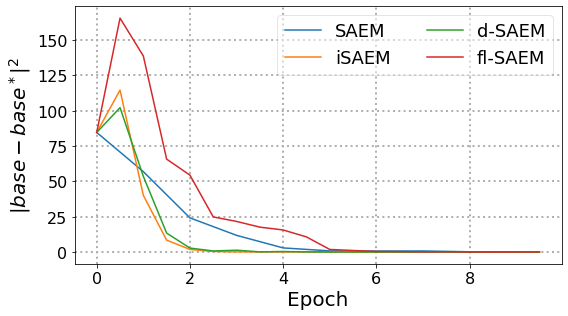
\includegraphics[width=\linewidth]{fig/flsaem_oxboys_mc.png}
   \caption{(Oxford Boys Dataset)}
\label{fig:resultstoy}
\end{figure}

\paragraph{Fitting a nonlinear mixed model on Warfarin dataset \citep{international2009estimation}}


\subsection{Probabilistic Latent Dirichlet Allocation}



\subsection{Bi-factor models under the Federated Learning settings}

\clearpage

\section{Conclusion}


\newpage

\bibliographystyle{abbrvnat}
\bibliography{ref}



%-----------------------------------------------------------------------------
%\vspace{0.4cm}

\end{document} 
